\section{Blockchain Architecture}
\subsection{Overview}
\begin{frame}{Quick Overview}
    \begin{itemize}
        \item \textit{Hyperledger Fabric}
        \item Full stack blockchain application.
        \item User roles tied to a blockchain
              certificate authority - \textit{X.509} certificates.
        \item On-chain \textit{CouchDB} for indexed blockchain queries.
        \item Distributed smart contracts.
    \end{itemize}
\end{frame}
\subsection{User Roles}
\begin{frame}{User Roles}
    \begin{itemize}
        \item Energy producers and certifiers are registered with the
              Hyperledger Fabric Certificate Authority (CA).
        \item Upon account registration, a producer is registered with the CA.
        \item Chaincode is called on behalf of a producer/certifier.
        \item Distributed smart contracts for account creation.
    \end{itemize}
\end{frame}
\begin{frame}{Producer Creation Example}
    \begin{adjustbox}{max totalsize={1\textwidth}{0.85\textheight},center}
        \includesvg[inkscapelatex=false]{photos/AccountCreation.svg}
    \end{adjustbox}
\end{frame}
\subsection{Carbon Sales}
\begin{frame}{Carbon Sales}
    \begin{itemize}
        \item A producer is allowed to sell a fungible token called
              \textit{Carboncoin}.
        \item Offer for sale of tokens is stored on the blockchain.
        \item Aim is to encourage distributed trading of carbon using the
              blockchain as an intermediary.
        \item The producer entirely drives the trading process.
    \end{itemize}
\end{frame}
\begin{frame}{Carboncoin Sale Example}
    \begin{adjustbox}{max totalsize={1\textwidth}{0.85\textheight},center}
        \includesvg[inkscapelatex=false]{photos/CreateSale.svg}
    \end{adjustbox}
\end{frame}
\begin{frame}{Viewing Offers}
    \begin{itemize}
        \item An on-chain \textit{CouchDB} index is warmed for retrieving offers.
              \begin{itemize}
                  \item Warming happens whenever a new block is cut.
              \end{itemize}
        \item Optional \textit{carbon reputation} is attached to an offer
              so producers can ethically purchase carbon.
        \item Carbon reputation assists with increasing market quality.
    \end{itemize}
\end{frame}
\begin{frame}{Retrieving Offers Example}
    \begin{adjustbox}{max totalsize={1\textwidth}{0.85\textheight},center}
        \includesvg[inkscapelatex=false]{photos/GetOffersNo.svg}
    \end{adjustbox}
\end{frame}
\subsection{Direct Market Interaction}
\begin{frame}{Direct Market Interaction}
    \begin{itemize}
        \item A producer can directly purchase
              \textit{Carboncoin} outside of the open market
              at an \textit{extra cost}.
        \item The user is given an on-chain offer token to purchase
              \textit{Carboncoin}.
        \item The price per token is calculated using the maximum offer on the
              open market.
        \item Each $x_i$ in Equation~\ref{eq:1} represents an active offer
              in the market.
    \end{itemize}
    \begin{equation}
        \text{Direct Offer} =
        \max \left(\left\langle x_1, x_2, \dots, x_n \right\rangle\right) + 50
        \label{eq:1}
    \end{equation}
\end{frame}
\begin{frame}{Direct Offer Creation Example}
    \begin{adjustbox}{max totalsize={1\textwidth}{0.85\textheight},center}
        \includesvg[inkscapelatex=false]{photos/directOffer.svg}
    \end{adjustbox}
\end{frame}
\subsection{ESG Certificates}
\begin{frame}{ESG Certificate Interaction}
    \begin{itemize}
        \item Market activity triggered by an ESG certifier recording
              carbon production.
        \item As a step in certificate creation, the certifier invokes
              the carbon market smart contract.
        \item Both the certifier and the carbon market exist on the
              same \textit{Hyperledger} channel.
        \item If the user does not have enough \textit{Carboncoin}
              to pay for production, then a debt is recorded.
    \end{itemize}
    \begin{figure}
        \caption{Channel Interaction}
        \centering
        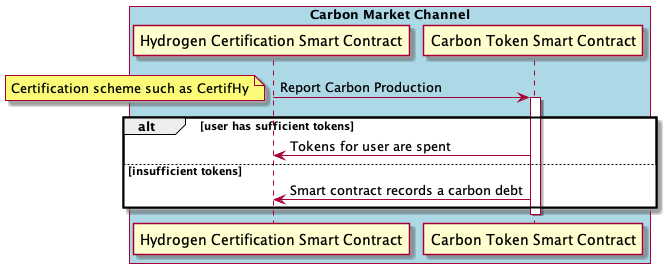
\includegraphics[height=0.5\textheight, width=0.5\linewidth,
            keepaspectratio]{photos/chain.png}
    \end{figure}
\end{frame}
